\documentclass[openany,11pt,a4paper]{report}

\usepackage{xcolor}
\usepackage{url}
\usepackage{array}
\usepackage{caption}
\usepackage{float}
%\usepackage{times}

  
\usepackage{amsmath} 
\usepackage{amssymb} 
\usepackage{bm}
\usepackage[colorlinks=true,breaklinks]{hyperref} 
\usepackage[hyphenbreaks]{breakurl} %
\usepackage{xcolor}
\definecolor{c1}{rgb}{0,0,1} % blue
\definecolor{c2}{rgb}{0,0.3,0.9} % light blue
\definecolor{c3}{rgb}{0.3,0,0.9} % red blue
\hypersetup{
linkcolor={c1}, 
citecolor={c2}, 
urlcolor={c3} 
}

\usepackage[nottoc]{tocbibind} 
\usepackage{graphicx}
\usepackage{longtable} 
\usepackage{bigstrut} 
\usepackage{enumerate}
\usepackage{todonotes} 
\usepackage{makeidx} 
\usepackage{color}


\usepackage{siunitx}
\usepackage{booktabs}




\usepackage{blindtext}

%% Math
\newcommand{\bra}[1]{\langle #1 | \,}
\newcommand{\ket}[1]{\, | #1 \rangle}
\newcommand{\braket}[2]{\langle #1 | #2 \rangle}



\makeindex

\usepackage[top=1.5cm, bottom=1.5cm,left=2.5cm,right=2.5cm]{geometry} % needed for page border settings
\parindent=0cm % for space of first line of new text block
\sloppy % for writing with hyphenless justification (tries to)
\hyphenation{} % use hyphenation of tolerance parameters, http://www.jr-x.de/publikationen/latex/tipps/zeilenumbruch.html
\hyphenpenalty=10000
\exhyphenpenalty=10000
\usepackage{fancyhdr}
%\usepackage[pdftex]{graphicx}
\usepackage{array,siunitx}



\begin{document}

\pagestyle{empty}


\begin{titlepage}

\newcommand{\HRule}{\rule{\linewidth}{0.5mm}} 
\center 

\textsc{\LARGE University of Cologne}\\[1.5cm]
\textsc{\Large Advanced Lab Course}\\[0.5cm] 

\vfill


\HRule \\[0.4cm]
{\huge \textbf {Experiment M2.6: Electron Spin Resonance}}

 
\vfill

\begin{minipage}{0.4\textwidth}
\begin{flushleft} \large
\emph{Group 27}\\
Panagiota \textsc{Kardala}\\
Rabia \textsc{Zahid} 
\end{flushleft}
\end{minipage}
~
\begin{minipage}{0.4\textwidth}
\begin{flushright} \large
\emph{Tutor:} \\
{Anudja } 
\end{flushright}
\end{minipage}\\[4cm]


\vfill

{\large \today}\\[3cm] 

\vfill

\end{titlepage}



\pagestyle{plain}

\tableofcontents







\begin{abstract}
In this experiment we studied the Electron Paramagentic Resonance (EPR) linewidths of a $CuSO_{4}\cdot 5H_{2}O$ crystal and powder sample, while a magnetic field is swept along the crystal's easy axis, at fixed excitation frequency. The goal was the measurement of the Lande g-factor, in order to extract its dependence on the orientation of the crystal. 
\end{abstract}


\chapter{Theoretical background}



\section*{Paramagnetism}
Paramagnetic ions have a permanent magnetic moment due to the coupling of their angular
momentum $\ell$ their electron spin $s$. The properties of the paramagnetic ions in crystal lattices are determined by their energy levels, that can be obtained by the calculation
of the energy levels of a free ion with further modifications, when the ion is placed at a
crystal lattice site.


\subsection{The spin-orbit coupling}


The electron has an internal magnetic moment $\vec{\mu_ {s}}$ connected with its intrinsic spin $\vec{s}$ through the relation $\vec{ \mu_ {e}} = g \mu_ {B}  \vec{s} $, where $ \mu_ {B} =  \dfrac{ -e \hbar}{2m_ {e} c} $ is a physical constant known as the Bohr magneton and $g$ is the Lande factor. An applied magnetic field $\vec{B}=- \dfrac{1}{c^{2}} \vec{v} \times \vec{E}$ can be expressed as $B= \dfrac{1}{m_{e}c^{2}e r} \dfrac{\partial V }{ \partial r} ( \vec{r} \times m_{e} \vec{v})=\dfrac{\hbar}{m_{e}c^{2}}\dfrac{1}{er} \dfrac{\partial V}{ \partial r} \vec{l}$ using the expression of the total angular momentum $\hbar \vec{l}= \vec{r} \times m_{e} \vec{v} $ and  $E=\dfrac{1}{e} \dfrac{\partial V}{ \partial r} \dfrac{\vec{r}}{r}$.\\

When the electron is placed in a constant
magnetic field $\vec{B}$, its magnetic moment couples to $\vec{B}$ through the interaction $H = - \vec{\mu_{s}} \cdot \vec{B}=-g \mu_{B} \vec{s} \vec{B} $.





Since the electron carries electric charge, its orbital motion around the nucleus is equivalent to an electric current, generating a magnetic moment called orbital magnetic moment $\vec{ \mu _{l}} = \mu_ {B} \vec{l}$.
This magnetic moment interacts with the spin magnetic moment and affects the
energies of the atomic levels obtained without consideration of
the spin.
The energy of interaction obtained through the Dirac equation is 
\begin{equation}
E= \frac{\hbar^{2}Ze^{2}}{2m_{e}^{2}c^{2}} \frac{\bm{l}\cdot \bm{s}}{4 \pi \varepsilon_{0} r^{3}} \label{eq:spinorbitint}
\end{equation}
with
\begin{equation}
\bm{l} \cdot \bm{s} = \dfrac{ j(j+1)-l(l+1) -s(s+1)}{2}
\end{equation}

where the two angular momenta, the orbital $l$ and the spin $s$, are coupled through a mutual interaction called spin-orbit coupling. Each of them has its own vector space but a complete description of the atom incorporating both requires the combination (tensor product) of the two spaces, thus we consider states of the form $\ket{nlm_{l}} \ket{sm_{s}}$. The vector operator $\bm{j} = \bm{l} + \bm{s}$ is an angular momentum operator which possesses eigenstates of the form $\ket{jm}$.
Combining the bases {$\vert l m_l\rangle$}   and {$\vert s m_{s}\rangle$}, we obtain a basis for the tensor product space where any state of the system is a linear combination of tensor products of the eigenstates of the form $\vert l m_{l}\rangle \vert s m_{s}\rangle$, equivalent to the basis of the eigenstates $\vert j,m\rangle$. The quantity $j$ is called total angular momentum and it can take values $ \mid l- s \mid \leq j \leq l+s$ in integer steps.  The two bases are related by a transformation matrix i.e. the Clebsch-Gordan coefficients $C_{m_{l},m_{s}}^{j}\equiv \langle l m_{l} ; sm_{s}\vert j, m \rangle $, thus we can finally express the eigenstates as
\begin{equation}
\vert j,m\rangle= \sum_{m_{l},m_{s}} C_{m_{l},m_{s}}^{j} \vert l m_{l}\rangle \vert sm_{s}\rangle
\end{equation}

The Clebsch-Gordan coefficients are non-zero only for values of $m_{l}$ and $m_{s}$ such that $m_{l} + m_{s} = m$. Each atomic state in a one-electron atom characterized by the
total angular momentum $j$. Each state $\vert nlm_{l}\rangle$ of the electron without spin when coupled with the spin states leads to two new states with total angular momenta $j = l + \frac{1}{2}$
and $j = l - 1/2$, with $m$-values according to the standard rules for angular momentum projection.
Thus a state $\vert nlm_{l} \rangle$ when combined with the electron spin gives rise to the states labelled as $\vert nlm_{l}; l+1/2,m \rangle$ and $\vert nlm_{l}; l- 1/2,m\rangle $. The principal quantum number $n$ is unaffected by the angular momentum and since the electron spin is always $s=\frac{1}{2}$, the spectroscopic notation is usually used, as $nl_j$.\\

The energy of the $nl_j$ states is shifted from the $nl$ states, typically the one with $j = l + 1/2$ upwards and $j = l - 1/2$ downwards. This change of energies, known as the fine structure splitting of the energy levels characterized by the same principal $n$ and orbital $l$ quantum numbers, is due to the interaction between the orbital and spin magnetic moments given by equation (\ref{eq:spinorbitint}).\cite{ls}\\                                                                                          

The atomic magnetic moment according to its orbital and spin contribution is expressed finally as
$ \vec{\mu } = \vec{ \mu_ {s}}  + \vec{ \mu _{l}}    = g \mu_ {B}  \vec{s} + \mu_ {B} \vec{l} $. The interaction of the atom with the external magnetic field is then described by $H_{Z}= - \vec{\mu} \vec{B}= (\vec{ \mu_ {s}}  + \vec{ \mu _{l}} ) \vec{B}$. The expectation value of this so called Zeeman interaction Hamiltonian is calculated in the $\vert j,m\rangle$ basis, considering it as a perturbation to the spin-orbit coupling interaction i.e. $E_{Z} \ll E_{SO}$.



\cite{foot}


\section{Spin Pairing energy}

There are two different types of spin paring configurations for an atom or ion: paramagnetic or diamagnetic. Paramagnetic and diamagnetic configurations result from the amount of d electrons in a particular atom. The energy associated with the spin pairing of these configurations relies on a factor of three things, the atom (for its electronic configuration and number of d electrons), the Crystal Field Theory (field splitting of electrons), and the type of ligand field complex (tetrahedral or octahedral).

Being diamagnetic means having all electrons paired and the individual magnetic effects cancel each other out. 
Being paramagnetic means having unpaired electrons and the individual magnetic effects do not cancel each other out. The unpaired electrons carry a magnetic moment that gets stronger with the number of unpaired electrons causing the atom or ion to be attracted to an external magnetic field.




According to Hund's Rule, it takes energy to pair electrons, therefore as electrons are added to an orbital, they do it in such a way that they minimize total energy; this causes the 2s orbital to be filled before the 2p orbital. When an electron can singly occupy a given orbital, in a paramagnetic state, that configuration results in high spin energy. However, when two electrons are forced to occupy the same orbital, they experience a interelectronic repulsion effect on each other which in turn increases the total energy of the orbital. The greater this repulsion effect, the greater the energy of the orbital.


Electron spin pairing energy transition from 2 unpaired electrons in two orbitals to 2 paired in one orbital is characterized by a decrease of the electronic repulsion. \cite{spinpairing}



\section{Crystal Field Theory (field splitting of electrons)}

Crystal field theory (CFT) describes the breaking of orbital degeneracy in transition metal complexes due to the presence of ligands. CFT qualitatively describes the strength of the metal-ligand bonds. Based on the strength of the metal-ligand bonds, the energy of the system is altered. This may lead to a change in magnetic properties as well as color. 
In Crystal Field Theory, it is assumed that the ions are simple point charges. When applied to alkali metal ions containing a symmetric sphere of charge, calculations of bond energies are generally quite successful. The approach taken uses classical potential energy equations that take into account the attractive and repulsive interactions between charged particles ( Coulomb's Law interactions)............\\\\\\



When examining a single transition metal ion, the five d-orbitals have the same energy. When ligands approach the metal ion, some experience more opposition from the d-orbital electrons than others based on the geometric structure of the molecule. Since ligands approach from different directions, not all d-orbitals interact directly. These interactions, however, create a splitting due to the electrostatic environment.



For example, consider a molecule with octahedral geometry. Ligands approach the metal ion along the x,y and z axes. Therefore, the electrons in the  dz2  and  dx2 y2 orbitals (which lie along these axes) experience greater repulsion. It requires more energy to have an electron in these orbitals than it would to put an electron in one of the other orbitals. This causes a splitting in the energy levels of the d-orbitals. This is known as crystal field splitting.


 \cite{CFT}

\section{Ligands}
A metal ion in solution does not exist in isolation, but in combination with ligands (such as solvent molecules or simple ions) or chelating groups, giving rise to complex ions or coordination compounds. Chelation is a process in which a polydentate ligand bonds to a metal ion, forming a ring. These complexes contain a central atom or ion, often a transition metal, and a cluster of ions or neutral molecules surrounding it. Ligands are ions or neutral molecules that bond to a central metal atom or ion. Ligands act as Lewis bases (electron pair donors), and the central atom acts as a Lewis acid (electron pair acceptor). Ligands have at least one donor atom with an electron pair used to form covalent bonds with the central atom. Ligands can be anions, cations, or neutral molecules. Ligands can be further characterized as monodentate, bidentate, tridentate etc. A monodentate ligand has only one donor atom used to bond to the central metal atom or ion. \cite{ligand}

\section{Crystal structure of $CuSO_{4}\cdot 5H_{2}O$}
The unit ce11 of copper sulfate contains two
$Cu^{++}$ ions, each surrounded by four negatively
charged oxygens (parts of water molecules)
in an approximate square, 2.8A on a side; there are
also two other oxygens (parts of sulfate groups),
each of which is 3.1A from any one of the oxygens
in the square. The six oxygens form an octahedron
about the cupric ion, where the body diagonal perpendicular to the square is the longest. The above arrangement produces an electric
field of nearly tetragonal symmetry at each
$Cu^{++} ion$ and the angle between the two tetragonal axes is close to $98^{o}$. \cite{crystalepr}



\begin{figure}[H]
\centering
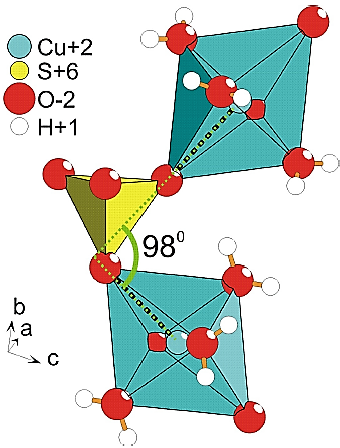
\includegraphics[scale=0.6]{cry.PNG}
\caption{A perspective view of the $CuSO_{4}\cdot 5H_{2}O$ structure with indicated angle (dashed
line) between the two Cu sites and their tetragonal axes. \cite{crystalepr}}
\end{figure}





\section{EPR in Copper sulphate.}

Using EPR in Copper sulphate, one can investigate  the separations of the lowest energy levels, correlated with the crystalline field theory for the particular ion, and the width of the absorption
line, giving information about the interactions of the ions with each other and with the lattice.
According to \cite{general}, using a single crystal  is more possible to obtain detailed information about the lowest energy levels of a paramagnetic ion, comparing to its powder.




Here we will compare our results with \cite{3.25sos}, where the same experiment was conducted for cavity frequency at $9.224 GHz$.


\subsection{Paramagnetic resonance: g-factor and the linewidth}  

Electron Spin Resonance (ESR) is used to study the magnetic properties of a material. Here, the oscillating magnetic field is applied to the crystal structure of $CuS0_{4}.5H_{2}O$  with a microwave frequency in order to remove the spin degeneracy which gives an energy difference equal to $g\beta H$. The paramagnetic absorption takes place when the energy of the incoming photon is equal to the energy difference between the spin levels which is given by, 
\begin{center}
$h\nu=g\beta H$
\end{center}
H is the magnetic field, $\beta$ is the Bohr magneton and the orientation of the magnetic field effects the g value. The magnetic field $H$ is varied but the frequency $\nu$ is remained constant. The absorption takes place when the resonance condition is satisfied. For $CuS0_{4}.5H_{2}O$ two different magnetic field values will be satisfied since there are two two $Cu^{++}$ ions which will give two g values. The g value is given by the equation,
\begin{center}
$g=\sqrt{(g_{\parallel}^{2}cos^{2}\theta+g_{\perp}^{2}sin^{2}\theta)}$
\end{center}
where, $\theta$ is the angle between the magnetic field and the tetragonal axis. 
According to the theory, the calculated value for $g_{\parallel}$ and $g_{\perp}$ is 2.06 and 2.47 respectively. \cite{general} 
Moreover, the wavelength and the direction of the magnetic field and also affect the width of the absorption line. Bagguley and Grifffiths noticed in their research that the line width was very small when the H was parallel to the tetragonal axis and it was not dependent on the wavelength. However, the line width increased with the decreasing wavelength when H was perpendicular to the axis. The width of the absorption line is affected because of different processes like spin-lattice interaction and spin-spin interaction. Gorter and Vleck also propose that the narrowing of the line widths can be due to the exchange of electrons between the $Cu^{++}$ ions. \cite{crystalepr} \\


Dipole-dipole and Super exchange interactions are also involved in shaping the curve of the spectrum. 


\subsection{Dipole-dipole interactions}


Dipole-dipole interaction is a magnetic phenomena. The local field of a magnetic dipole is felt by another dipole in a modified way and the resonance is shifted which results in the broadness of the spectrum. This interaction is depended on the distance r which is given by,
\begin{center}
$H_{loc}=\dfrac{\mu_{B}}{4 \pi r^{3}}$
\end{center}
It also depends on the orientation of the adjacent spins which also changes the shape of the curve. A Gauss or a Lorentz line shape is observed depending on the type of spin interaction. When the spins are dissimilar the interaction results in a Gauss like curve because of the uniform dipole fields which results in inhomogeneous broadening. However, similar spins results in a Lorentz like curve because of the dynamic homogeneous broadening.   
\\


\subsection{Exchange interactions}

The line shape is influenced by spin-spin exchange interaction over a specific number of spins in paramagnetic materials. The Pauli exclusion principle is responsible for the exchange interactions which is is triggered because of the superposition of the electron wave functions. The superposition of two paramagnetic atoms which are next to each other lead to a direct exchange. Whereas,indirect exchange or super exchange occurs when there is a diamagnetic atom between two paramagnetic atoms. This kind of interaction is also explained by the coherence phenomena which says that that the superposition of wave functions decreases the frequencies because of the similar fields $H_{loc}$ and it gives a Lorentz like curve shape.  \\


The line shape of the resonance curve can be affected by both dipole dipole an exchange interactions if the magnetic moments of the spins are not similar and the curve shape then depends on the interaction which is more stronger. 



\section{gfator derivation}

the g parallel comes from the z axis when we see the molecule structure, while the perpendicular from the x-y plane 



\section{bumps}
the unexpected/assymetric bump that we observe is  the residual is due to spin
exchange and, in fact, yields an independent method to
estimate the spin exchange frequency. According to
all theories the eigenvalues of the spin exchange spin
Hamiltonian are complex, which implies that the lineshape
of the spin exchange broadened EPR line is no
longer purely Lorentzian. \cite{bump}


\chapter{Procedure and Analysis}
We measured firstly the relation of the angle between the main axis and the applied magnetic field for the crystal, in order to extract the $g$ values, in steps of $10 ^{o}$. Before every measurement, we checked that the frequency of the cavity is tuned in steady state and made sure that the lock offset is zero, while the magnetic field was in "tune mode". Finally we performed a DC scan of the applied magnetic field, every time starting from $-4000 Gs$ to $-2000Gs$, in order to avoid the Hysteresis phenomenon.\\


We fitted the spectra acquired for each angle according to the first derivative of the Lorentzian and Gaussian functions, where we identified the peaks position on x-axis for each case, to obtain the $g_{\perp}, g_{\parallel}$ values as indicated in \cite{viscous_liquids} according to Fig \ref{Fig:reference}, using  $g=  \dfrac{h \nu}{\mu_{B} H}$.




\begin{figure}[hbtp]
\caption{\cite{viscous_liquids}}
\centering
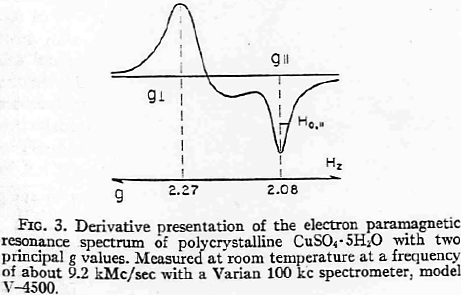
\includegraphics[scale=0.9]{analzsis.PNG}
\label{Fig:reference}
\end{figure}



The first derivative of a Lorentzian curve that we used to fit our data is given by

\begin{equation}
y=-\dfrac{ y_{0} \gamma (x-a)}{\pi [ \dfrac{\gamma ^2}{4}  + (x-a)^2]^2}
\label{eq:Lorentzian}
\end{equation}

where $\alpha$ is the zero point of the derivative, $\gamma $ and $\sigma$ are functions of the width at FWHM and $y_{0}$ is the offset factor required for the optimisation of our fits .\\

Respectively the first derivative of a Gaussian curve used is 
\begin{equation}
y=-\dfrac{y_{0}(x-a)e^{-\dfrac{(x-a)^2}{2\sigma ^2}}}{\sqrt{2 \pi } \sigma ^3}
\label{eq:Gaussian}
\end{equation}

The FWHM is given by $\gamma $ for the Lorentzian  fits and by $2.355 \cdot \sigma$ for the Gaussian.\\



For the $g$ calculation we used : $h= 4.135667 \cdot 10^{-15} eV \cdot sec$, $\mu_{B} = 5.788381 \cdot 10^{-5} eV\cdot T$.\\

Throughout the crystal measurements the frequency was stable at $\nu_{c}= 9.47 GHz$, while during the powder measurements at $\nu_{p}= 9.48 GHz$. The experiment was conducted in room temperature.

\begin{table}[H]
\centering
\caption{Lorentzian fit of the crystal's data.}
\noindent\begin{tabular}{| l || S | S | S || S | S | S |}
\cline{2-7}
\multicolumn{1}{c|}{}& \multicolumn{6}{c|}{Lorentzian}   \\
\hline
$\theta (\pm 2^{o}) $ & {$H_{p,l}$ (Gs)} & {$g_{\perp}$} & {$\delta g_{\perp}$} & {$H_{p,r}$ (Gs)}  & {$g_{\parallel}$} & {$\delta g_{\parallel}$}  \\
\hline

10 & -3174.89
 & 2.1311 & 0.0008
 & -3085.46
 & 2.1929 & 0.0009 \\
20 & -3186.14
 & 2.1236 & 0.0008
  & -3108.85 & 2.1764
 & 0.0009 \\
30 & -3195.19
 & 2.1176 & 0.0008 & -3131.57
 & 2.1606 & 0.0009 \\
40 & -3201.23
 & 2.1136 & 0.0008 & -3144.9
 & 2.1515 & 0.0008 \\
50 & -3200.59
 & 2.1140 & 0.0008 & -3146.74
 & 2.1502 & 0.0008 \\
60 & -3195.25
 & 2.1175 & 0.0008 & -3130.04
 & 2.1572 & 0.0009 \\
70 & -3185.58
 & 2.1240 & 0.0008 & -3116.47 & 2.1711 & 0.0009 \\
80 & -3175.35
 & 2.1308 & 0.0008 & -3089.77 & 2.1898 & 0.0009 \\
90 & -3157.53 
 & 2.1428 & 0.0008 & -3056.32 & 2.2138 & 0.0009 \\
100 & -3143.01
 & 2.1527 & 0.0009 & -3027.08 & 2.2352 & 0.0009 \\
110 & -3121.53
 & 2.1676 & 0.0009 & -3006.82
 & 2.2503 & 0.0009 \\
120 & -3111.13
 & 2.1748 & 0.0009 & -2990.81
 & 2.2623 & 0.0009 \\
130 & -3101.09
 & 2.1818 & 0.0009 & -2983.68 & 2.2677 & 0.0009 \\
140 & -3096.63 & 2.1850 & 0.0009 & -2983.55 & 2.2678 & 0.0009 \\
150 & -3097.65 & 2.1843 & 0.0009 & -2990.96 & 2.2622 & 0.0009\\
160 & -3102.95
 & 2.1805 & 0.0009 & -3003.79 & 2.2525 & 0.0009 \\
170 & -3121.64
 & 2.1675 & 0.0009 & -3025.44 & 2.2364 & 0.0009 \\
190 & -3152.53
 & 2.1462 & 0.0008 & -3068.91
 & 2.2047 & 0.0009 \\
 200 & -3187.68 & 2.1226 & 0.0008 & -3113.13
 & 2.1734 & 0.0009   \\

\hline
\end{tabular}
\label{Tab:peaks}
\end{table}


\begin{table}[H]
\centering
\caption{Gaussian fit of the crystal's data.}
\noindent\begin{tabular}{| l || S | S| S || S | S | S |}
\cline{2-7}
\multicolumn{1}{c|}{}& \multicolumn{6}{c|}{Gaussian} \\
\hline
$\theta (\pm 2^{o}) $ & {$H_{p,l}$ (Gs)} & {$g_{\perp}$} & {$\delta g_{\perp}$} & {$H_{p,r}$ (Gs)} & {$g_{\parallel}$} & {$\delta g_{\parallel}$}  \\
\hline

10 & -3197.46
 & 2.1161 & 0.0008 & -3075.97 & 2.1997 & 0.0009 \\
20 & -3200.34
 & 2.1142 & 0.0008 & -3101.03 & 2.1819 & 0.0009 \\
30 & -3204.12
 & 2.1117 & 0.0008 & -3124.88 & 2.1652 & 0.0009 \\
40 & -3208.83 & 2.1086 & 0.0008 & -3138.48 & 2.1559 & 0.0009 \\
50 & -3208.39
 & 2.1089 & 0.0008 & -3140.47 & 2.1545 & 0.0009 \\
60 & -3203.91
 & 2.1118 & 0.0008 & -3130.04 & 2.1617 & 0.0009 \\
70 & -3196.51
 & 2.1167 & 0.0008 & -3109.41 & 2.1760 & 0.0009 \\
80 & -3191.38 & 2.1201 & 0.0008 & -3080.43 & 2.1965 & 0.0009 \\
90 & -3181.77 & 2.1265 & 0.0008 & -3043.65 & 2.2230 & 0.0009 \\
100 & -3170.54 & 2.1341 & 0.0008 & -3014.45 & 2.2446 & 0.0009 \\
110 & -3157.32 & 2.1430 & 0.0008 & -2993.3 & 2.2604 & 0.0009 \\
120 & -3148.92 & 2.1487 & 0.0008 & -2977.93 & 2.2721 & 0.0009 \\
130 & -3133.36 & 2.1594 & 0.0009 & -2971.43 & 2.2771 & 0.0009 \\
140 & -3120.04 & 2.1686 & 0.0009 & -2971.98 & 2.2766 & 0.0009 \\
150 & -3120.05
 & 2.1686 & 0.0009 & -2979.75 & 2.2707 & 0.0009 \\
160 & -3124.31
 & 2.1656 & 0.0009 & -2992.61 & 2.2609 & 0.0009 \\
170 & -3135.62
 & 2.1578 & 0.0009 & -3014.42 & 2.2446 & 0.0009 \\
190 & -3168.77
 & 2.1352 & 0.0008 & -3058.18 & 2.2125 & 0.0009 \\
200 & -3199.95
 & 2.1144 & 0.0008 & -3105.74 & 2.1786 & 0.0009 \\
\hline
\end{tabular}
\label{Tab:peaks}
\end{table}




For the $g$ calculation we used : $h= 4.135667 \cdot 10^{-15} eV \cdot sec$, $\mu_{B} = 5.788381 \cdot 10^{-5} eV\cdot T$.\\



Further we calculate the total $g$ values for each angle according to 
\begin{equation}
g= \sqrt{g^{2}_{\parallel}  cos^{2}\theta + g^{2}_{\perp} sin^{2}\theta}
\end{equation}



\begin{table}[H]
\centering
\caption{calculated g values.}
\noindent\begin{tabular}{| l || S | S || S| S | }
\cline{2-5}
\multicolumn{1}{c|}{} & \multicolumn{2}{c|}{Lorentzian} & \multicolumn{2}{c|}{Gaussian} \\
\hline
$ \theta (\pm 2 ^{o}) $ & {g} & {$\delta$ g} &  {g} & {$\delta$ g} \\
\hline
10 & 2.1161 & 0.2749 & 2.1753 & 0.5067 \\
20 & 2.1142 & 0.1287 & 2.1256 & 0.2108 \\
30 & 2.1117 & 0.0139 & 2.1130 & 0.0216
 \\
40 & 2.1086 & 0.1132 & 2.1297
& 0.1783 \\
50 & 2.1089 & 0.0203 & 2.1514
 & 0.0370 \\
60 & 2.1118 & 0.0344 & 2.1571 & 0.0634 \\
70 & 2.1167 & 0.1772 & 2.1407 & 0.2818 \\
80 & 2.1201 & 0.0141 & 2.1211 & 3.914 \\
90 & 2.1265
 & 6.561 & 2.1462 & 4.543 \\
100 & 2.1341 & 9.817 & 2.2167 & 6.061 \\
110 & 2.1430 & 12.743 & 2.2602 & 8.553 \\
120 & 2.1594 & 12.233 & 2.1756 & 8.258 \\
130 & 2.1686 & 13.828 & 2.1729 & 9.115 \\
140 & 2.1686 & 13.742 & 2.2191 & 8.580 \\
150 & 2.1656 & 10.535 & 2.2564 & 6.814 \\
160 & 2.1578 & 12.089 & 2.2343 & 7.473 \\
170 & 2.1352 & 8.430 & 2.1356 & 7.506 \\
190 & 2.1352 & 5.147 & 2.1356 & 3.697 \\
200 & 2.1144 & 3.968 & 2.1298 & 2.531 \\
\hline
\end{tabular}
\label{Tab:FWHM}
\end{table}


\begin{figure}[hbtp]
\centering
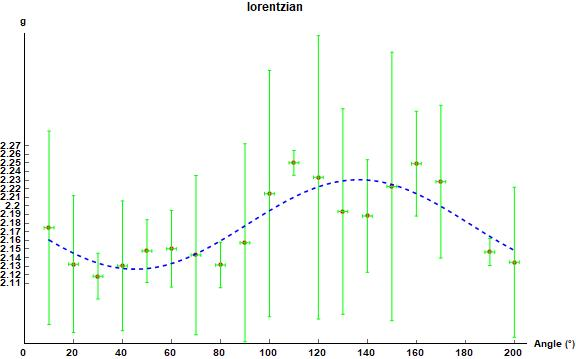
\includegraphics[scale=0.8]{glor1.jpg}
\caption{Fitted g-values, extracted from the Lorentzian approximation.}
\end{figure}




\begin{figure}[hbtp]
\centering
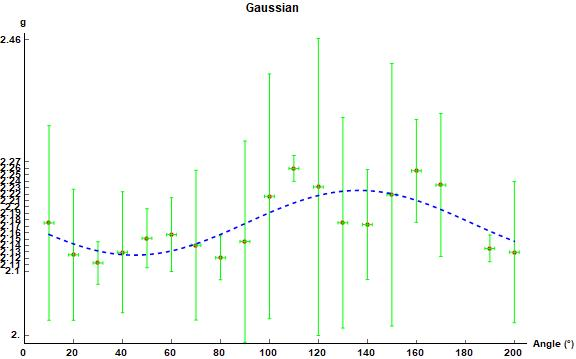
\includegraphics[scale=0.8]{ggau1.jpg}
\caption{Fitted g-values, extracted from the Gaussian approximation.}
\end{figure}

The data were fitted according to the function $g= a\cdot cos^{2}(n\cdot \theta + c) + e$, where we obtained $adj R^{2}_{Lor}=0.999857$ and $adj R^{2}_{Gau}=0.999748$.

\begin{table}[H]
\centering
\caption{FWHM}
\noindent\begin{tabular}{| l || S | S || S| S | }
\cline{2-5}
\multicolumn{1}{c|}{}& \multicolumn{2}{c|}{Lorentzian} & \multicolumn{2}{c|}{Gaussian} \\
\hline
 $ \theta (\pm 2 ^{o}) $ & {FWHM} & {$\delta _{FWHM}$} &  {FWHM} & {$\delta _{FWHM}$} \\
\hline
10 & 154.891 & 6.991 & 143.056 & 4.462 \\
20 & 133.868 & 4.863 & 116.942 & 3.071 \\
30 & 110.189 & 4.466 & 93.299 & 2.718 \\
40 & 97.563 & 4.329 & 82.846
& 2.539 \\
50 & 93.279 & 3.813 & 79.973 & 2.231 \\
60 & 101.791 & 4.019 & 86.984 & 2.394 \\
70 & 119.710 & 5.099 & 102.569 & 3.267 \\
80 & 148.237 & 5.671 & 130.638 & 3.914 \\
90 & 175.296 & 6.561 & 162.641 & 4.543 \\
100 & 200.791 & 9.817 & 183.800 & 6.061 \\
110 & 198.684 & 12.743 & 193.124 & 8.553 \\
120 & 208.397 & 12.233 & 201.345 & 8.258 \\
130 & 203.367 & 13.828 & 190.670 & 9.115 \\
140 & 195.872 & 13.742 & 174.344 & 8.580 \\
150 & 184.803 & 10.535 & 165.204 & 6.814 \\
160 & 171.764 & 12.089 & 155.081 & 7.473 \\
170 & 166.628 & 8.430 & 150.479 & 7.506 \\
190 & 144.846 & 5.147 & 130.220 & 3.697 \\
200 & 129.122 & 3.968 & 110.921 & 2.531 \\
\hline
\end{tabular}
\label{Tab:FWHM}
\end{table}







\begin{figure}[H]
\centering
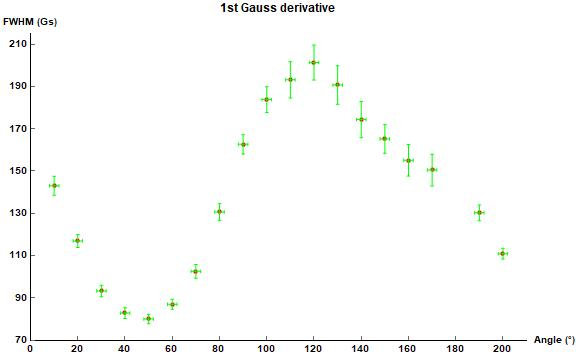
\includegraphics[scale=0.7]{fwhmgauss.jpg}
\caption{FWHM dependance on the angle change, for the Gaussian fits.}
\end{figure}




\begin{figure}[H]
\centering
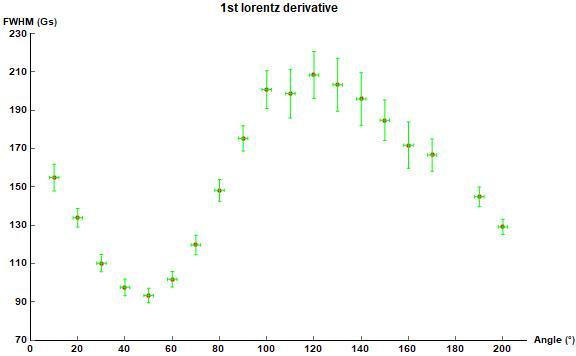
\includegraphics[scale=0.7]{fwhmlore.jpg}
\caption{FWHM dependance on the angle change, for the Lorentzian fits.}
\end{figure}




According to \cite{general}, for wavelength $9.86 GHz$ only one absorption line should be observed (concerning the dependance on the magnetic field, not its derivative). We expected asymmetric peaks because of the Brownian rotation effect on the absorption curves, i.e. the contribution to the spin-lattice relaxation and the spin-spin interaction,  \cite{viscous_liquids} , but as illustrated in the spectra bellow, the asymmetry is much larger than the expected. The maximum adjusted $R^{2}$ value for the fits is 0.861, which indicates a not so accurate approximation.



\begin{figure}[H]
\centering
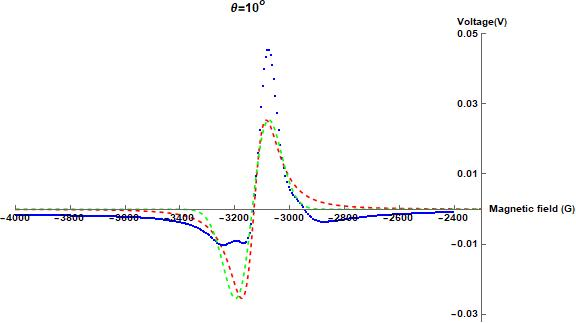
\includegraphics[scale=0.6]{10.jpg}
\end{figure}




\begin{figure}[H]
\centering
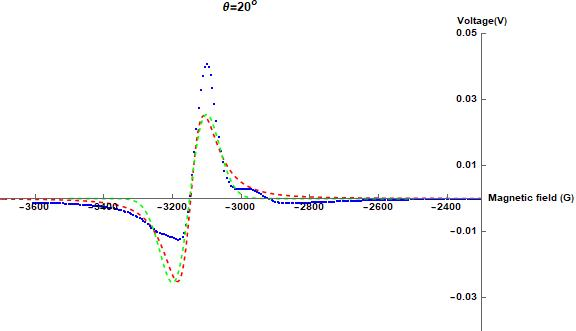
\includegraphics[scale=0.6]{20.jpg}
\end{figure}




\begin{figure}[H]
\centering
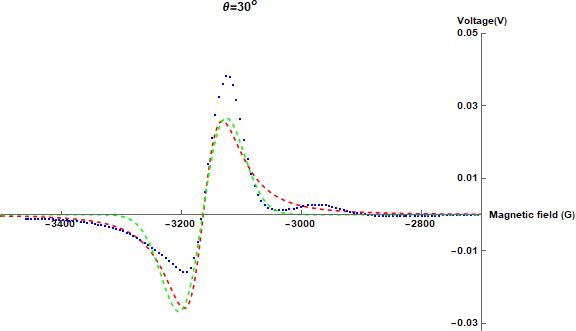
\includegraphics[scale=0.6]{30.jpg}
\end{figure}





\begin{figure}[H]
\centering
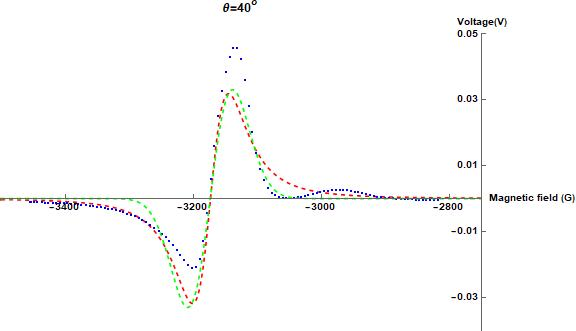
\includegraphics[scale=0.6]{40.jpg}
\end{figure}





\begin{figure}[H]
\centering
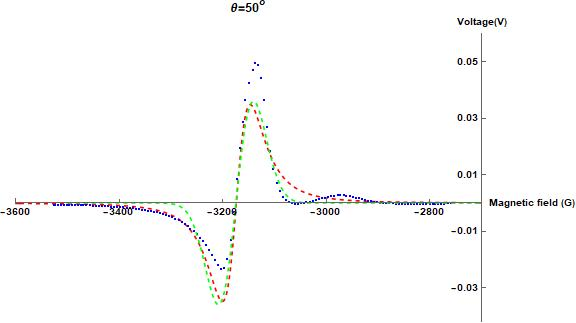
\includegraphics[scale=0.6]{50.jpg}
\end{figure}






\begin{figure}[H]
\centering
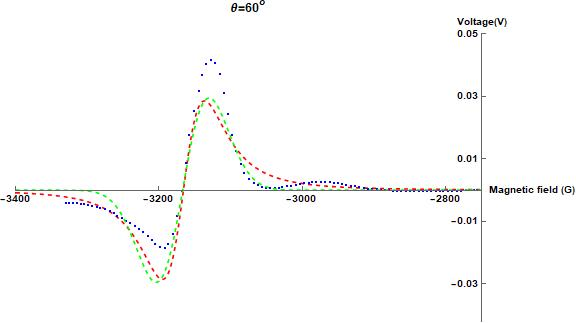
\includegraphics[scale=0.6]{60.jpg}
\end{figure}





\begin{figure}[H]
\centering
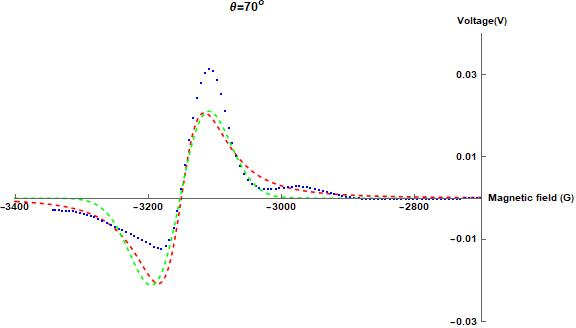
\includegraphics[scale=0.6]{70.jpg}
\end{figure}





\begin{figure}[H]
\centering
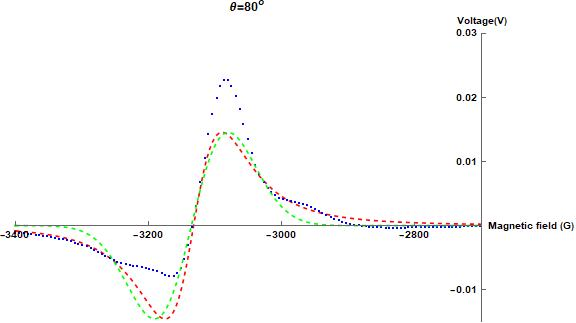
\includegraphics[scale=0.6]{80.jpg}
\end{figure}





\begin{figure}[H]
\centering
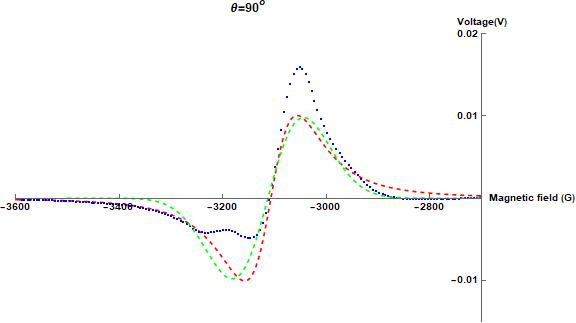
\includegraphics[scale=0.6]{90.jpg}
\end{figure}






\begin{figure}[H]
\centering
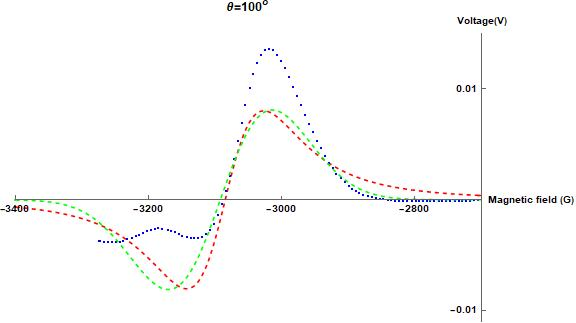
\includegraphics[scale=0.6]{100.jpg}
\end{figure}





\begin{figure}[H]
\centering
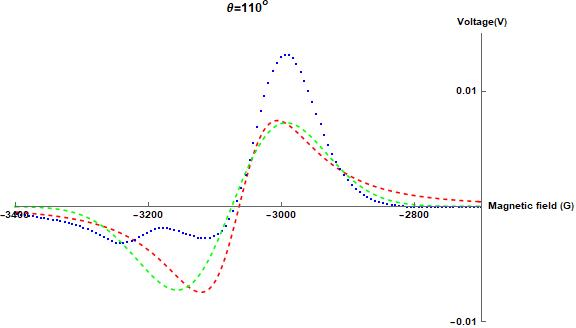
\includegraphics[scale=0.6]{110.jpg}
\end{figure}





\begin{figure}[H]
\centering
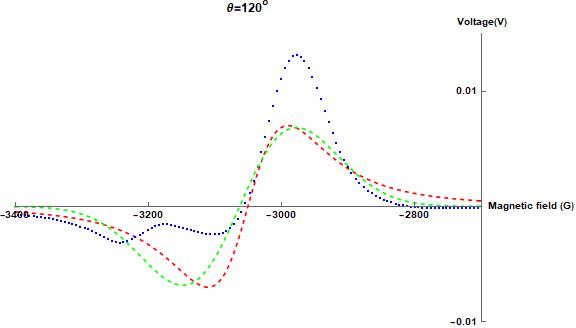
\includegraphics[scale=0.6]{120.jpg}
\end{figure}




\begin{figure}[H]
\centering
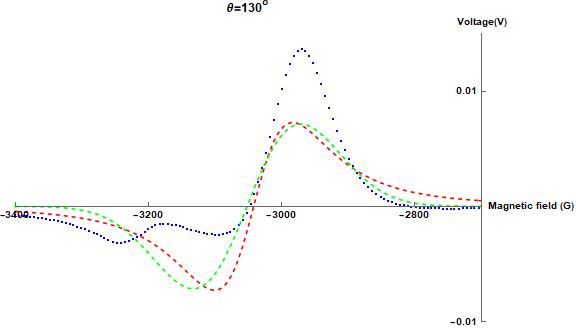
\includegraphics[scale=0.6]{130.jpg}
\end{figure}


\begin{figure}[H]
\centering
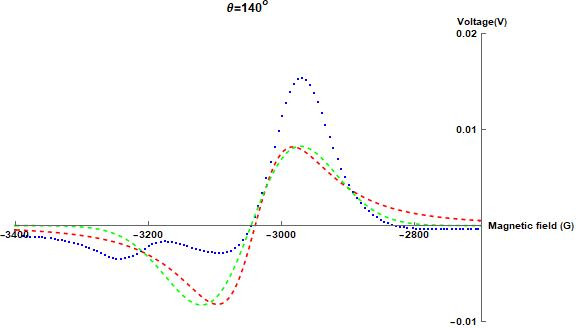
\includegraphics[scale=0.6]{140.jpg}
\end{figure}


\begin{figure}[H]
\centering
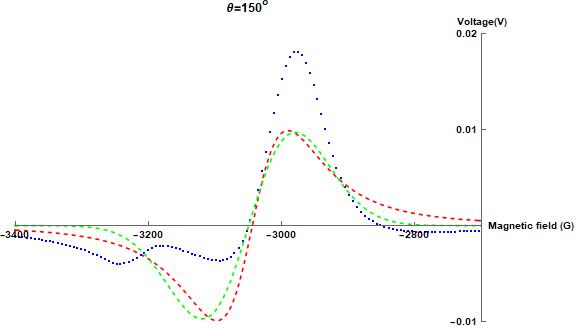
\includegraphics[scale=0.6]{150.jpg}\end{figure}


\begin{figure}[H]
\centering
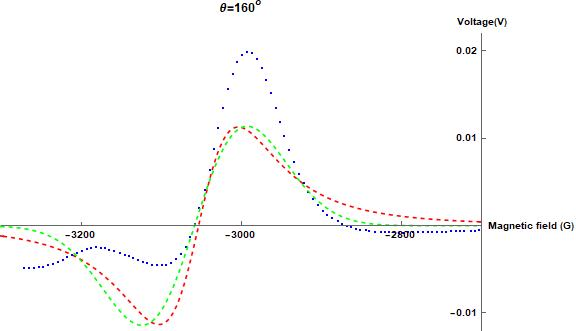
\includegraphics[scale=0.6]{160.jpg}
\end{figure}


\begin{figure}[H]
\centering
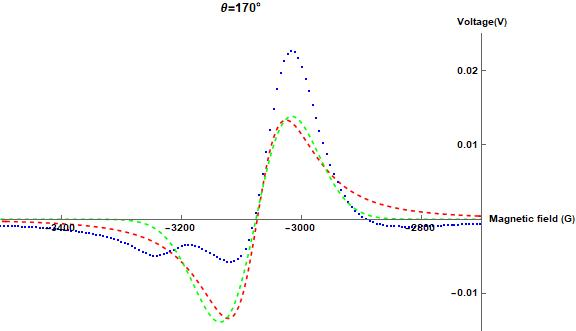
\includegraphics[scale=0.6]{170.jpg}
\end{figure}


\begin{figure}[H]
\centering
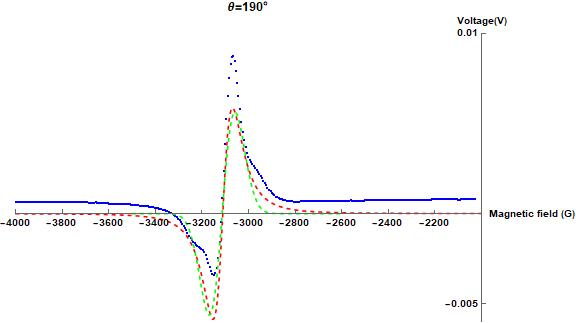
\includegraphics[scale=0.6]{190.jpg}
\end{figure}


\begin{figure}[H]
\centering
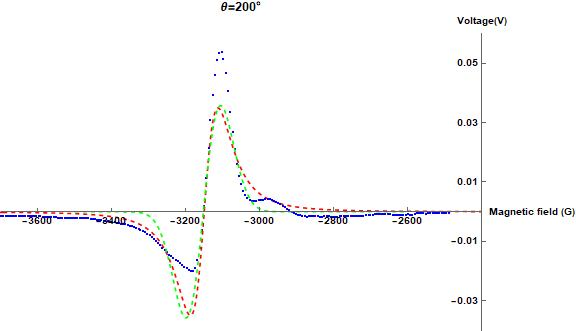
\includegraphics[scale=0.6]{200.jpg}
\end{figure}

\section{Reversed way}

Because the plots illustrating the calculated g values do not agree with the expected symmetric behaviour of \cite{3.25sos}, we decided to extract the g values by substituting the position of the zero of the first derivative of the magnetic field $a$ at H.


\begin{figure}[H]
\centering
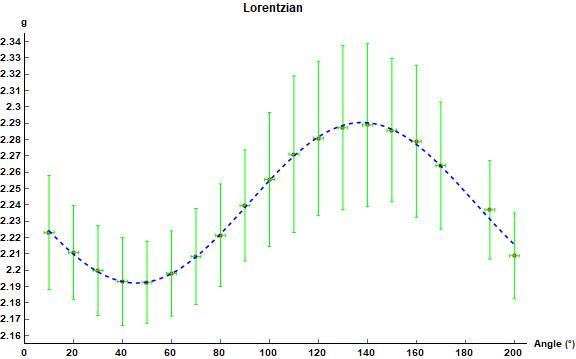
\includegraphics[scale=0.8]{glo2.jpg}
\caption{ $R^{2}=0.999999$}
\end{figure}



\begin{figure}[H]
\centering
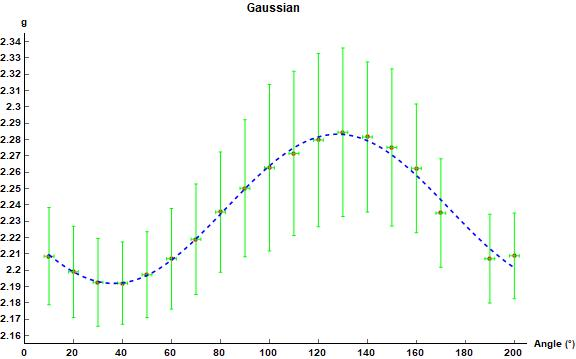
\includegraphics[scale=0.8]{gga2.jpg}
\caption{$R^{2}=0.999997$}
\end{figure}


We observe that data follow to the maximum the function $g= a\cdot cos^{2}(n\cdot \theta + c) + e$.



\subsection{Powder sample}
The powder sample spectra is just noise, either because the powder sample went bad, or because we misplaced the sample in the magnet. Thus we cannot perform any further analysis.



\begin{figure}[hbtp]
\centering
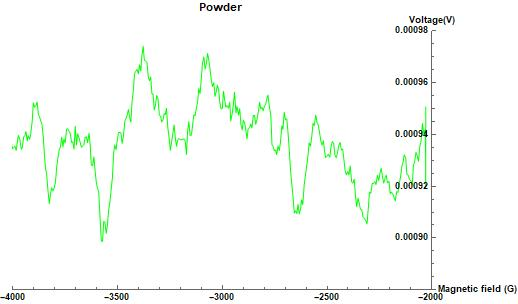
\includegraphics[scale=0.8]{powder.jpg}
\caption{•}
\end{figure}





\begin{thebibliography}{99}

\bibitem{3.25sos}  "Paramagnetic Resonance Absorption in Two Sulfates of Copper".
RGBERT D. ARNQLD AND ARTHUR F. KIP \url{https://journals.aps.org/pr/pdf/10.1103/PhysRev.75.1199}

\bibitem{spinpairing} \url{https://chem.libretexts.org/Bookshelves/Physical_and_Theoretical_Chemistry_Textbook_Maps/Supplemental_Modules_(Physical_and_Theoretical_Chemistry)/Electronic_Structure_of_Atoms_and_Molecules/Electronic_Configurations/Spin_Pairing_Energy?fbclid=IwAR3GAHSooUR1RbBXcl5AQKjqFIG9xzg95XFX84XP_tAGibb2fQyCa1Lj3YU}

\bibitem{ligand} \url{https://chem.libretexts.org/Bookshelves/Inorganic_Chemistry/Supplemental_Modules_(Inorganic_Chemistry)/Coordination_Chemistry/Structure_and_Nomenclature_of_Coordination_Compounds/Ligands}



\bibitem{CFT} \url{https://chem.libretexts.org/Bookshelves/Inorganic_Chemistry/Supplemental_Modules_(Inorganic_Chemistry)/Crystal_Field_Theory/Crystal_Field_Theory}





\bibitem{olo} \url{http://tuprints.ulb.tu-darmstadt.de/698/1/mestric_thesis.pdf}



\bibitem{ls} Lambropoulos Peter and Petrosyan David. 2007. Fundamentals of Quantum Optics and Quantum Information.  Berlin Heidelberg: Springer-Verlag. 211-282.\\
\url{https://doi.org/10.1007/978-3-540-34572-5}


\bibitem{general}Bagguley, D. M. S., and J. H. E. Griffiths. “Paramagnetic Resonance in Copper Sulphate.” Proceedings of the Royal Society of London. Series A, Mathematical and Physical Sciences, vol. 201, no. 1066, 1950, pp. 366–377. JSTOR, www.jstor.org/stable/98379. 
\url{https://www.jstor.org/stable/98379?seq=1#page_scan_tab_contents}


\bibitem{lineshapeg} Line Shapes in Electron Spin Resonance, Charles P. Poole and Horacio A. Farach, Department of Physics and Astronomy
University of South Carolina
Columbia, SC 29208, USA.  \url{https://www.weizmann.ac.il/ISMAR/sites/ISMAR/files/bulletin/BMR_01_162-194_1979.pdf}

\bibitem{isws} Line Shapes in Electron Spin Resonance Spectra,
J. Chem. Phys. 41, 949 (1964)
\url{ https://doi.org/10.1063/1.1726038}

\bibitem{viscous_liquids} 

Fritz Kurt Kneubühl. "Line Shapes of Electron Paramagnetic Resonance Signals Produced by Powders, Glasses, and Viscous Liquids". 1960. The Journal of Chemical Physics. Pages 1074-1078, VI  - 33, IP  - 4, AID  - 10.1063/1.1731336 [doi].
 The Journal of Chemical Physics 33:4, 1074-1078
\url{https://aip.scitation.org/doi/10.1063/1.1731336}


\bibitem{crystalepr}

John Wheatley and David Halliday. "Paramagnetic Absorption in Single Crystals of Copper Sulfate Pentahydrate". Phys. Rev. 75, 1412 – Published 1 May 1949. Vol. 75, Iss. 9
\url{https://doi.org/10.1103/PhysRev.75.1412}


\bibitem{bump}  Lineshapes of spin exchange broadened EPR spectra
Miroslav Peric* and Barney L. Bales
Department of Physics and Astronomy and the Center for Supramolecular Studies, California State University at Northridge, Northridge,
CA 91330, USA
Received 11 February 2004; revised 25 March 2004

\bibitem{foot} Foot, Atomic physics.


\end{thebibliography}






\end{document}
